\documentclass[12pt]{article}

\usepackage{graphicx}
\graphicspath{{figures/}} % Location of the graphics files
\usepackage[font=small,labelfont=bf]{caption} % Required for specifying captions to tables and figures
\usepackage{amsfonts, amsmath, amsthm, amssymb}
%\usepackage{wrapfig}
\usepackage{indentfirst}

\begin{document}
\title{HAPIEST User Manual} 
\date{}
\maketitle
\thispagestyle{empty}
\newpage

\tableofcontents
\thispagestyle{empty}
\newpage

\setcounter{page}{1}
\section{HAPIEST}
HITRAN Application Programming Interface and Efficient Spectroscopic Tools (HAPIEST) is a GUI for the HITRAN Application Programming Interface. HAPIEST started development at SUNY Oswego in a software engineering course by students Benji Caro, Joshua Karns, Dominik Lohmann, Wyatt Matt, Ethan Messer, and Michael Sova,a dn in conjunction with Dr. Iouli Gordon and Dr. Roman Kochanov of the Harvard-Smithsonian Center for Astrophysics and under advisement of SUNY Oswego professor Bastian Tenbergen and SUNY OSwego Professors and Head of Physics Department Shashi Kanbur. HAPIEST functions as a GUI for the HITRAN Application Programming Interface.
\subsection{Program Overview}
The goal of HAPIEST is to simplify the use of the HITRAN Application Programming Interface (HAPI) for all users. Currently, HAPI requires some knowledge of Python and use of the command line. HAPIEST should retain as much of the funtionality HAPI as is possible in a simple GUI, while making it easier to access and use for the user. HAPIEST currently allows users the capability to fetch/download and locally store data from the HITRAN database, edit local data, and also to generate and plot spectral functions. In it's current form, HAPIEST is split up into 3 windows, one window for data management and editing, and two windows for graphing/graph display.
\section{How to Use}
\subsection{Fetching Data}
In order to plot/graph data, the user needs to first download data from the HITRAN database. This can be done in HAPIEST or using HAPI. To do so in HAPIEST, follow the instructions below.
\begin{enumerate}
\item Edit data name to change the name of the file downloaded upon fetching.
\item Select the molecule to update the Isotopologues list.
\item Select the Isotopologues you want to download data for.
\item Select from the Parameter Groups and Parameters list to download further data for the selected Isotopologues.
\item Edit the Wave Number Min and Max values to refine your download (Smaller ranges are faster to fetch and take up less space).
\end{enumerate}

\subsection{Graphing Data}
Once you have data on your system, you can then go to the Graphing Tab to produce a graph. 
\begin{enumerate}
\item In the Data Name list, select the data file you want to use to create a plot.
\item Skip Draw in Existing Window for now, and select the parameters of the plot.
\item Click the graph button and another window will appear to display the graph.
\item Now, if you want to plot another graph of the same type in/with a previous plot, check the Draw in Existing Window check box and select the compatible window in the drop-down list.
\end{enumerate}

\section{Main Window}
The Main Window provides the functionality of HAPI and is split into several tabs each focusing on a different feature/function. 
\subsection{Fetch Tab}
The Fetch tab allows the user to download data from HITRAN onto their local disk for the available molecules and their supported isotopologues. Further, the user can select from the \textit{Parameter Groups} list and \textit{Parameters} list to download more specific data. This window is the users primary method of obtaining data.
\begin{center}
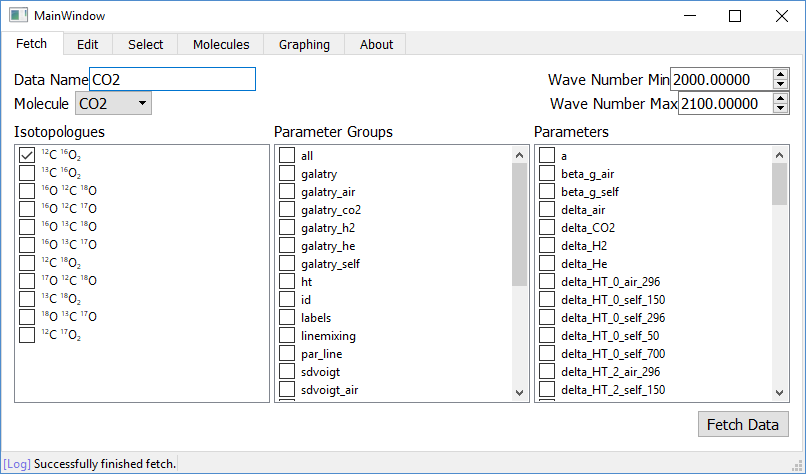
\includegraphics[scale = 0.8]{MainWindow_Fetch}
\end{center}
\subsubsection{Element Dictionary}
\begin{itemize}
\item Data Name - Local file name of data being downloaded.
\item Molecule - List of molecules to select which Isotopologues to fetch data for, updates the Isotopologues list when a molecule is selected.
\item Wave Numer Min - Lower threshold to fetch data (from).
\item Wave Number Max - Upper threshold to fetch data (to).
\item Isotopologues - List of Isotopologues for the selected molecule, these are what you are fetching data for.
\item Parameter Groups - List containing groups of parameters. Select from these groups to add parameters to the fetch.
\item Parameters - List of specific (un-grouped) parameters. Select from these parameters to add them to the fetch.
\end{itemize}

\subsection{Edit Tab}
\begin{center}
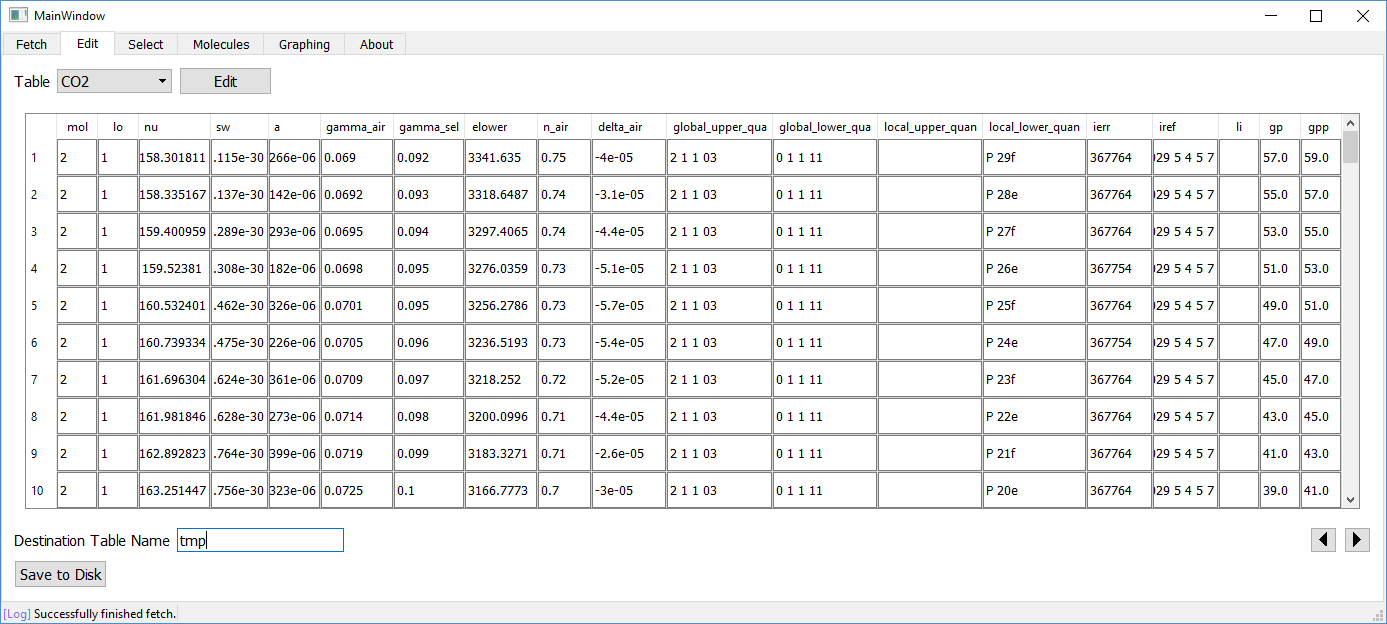
\includegraphics[scale = 0.4]{MainWindow_Edit}
\end{center}
\subsubsection{Element Dictionary}
\begin{itemize}
\item Table - List of HITRAN data files.
\item Edit - Button that populates table containing information in the data file.
\item Destination Table Name - Name of local file upon saving.
\item (Left and Right Arrows) - Select between pages of data.
\item Save to Disk - Button that saves the  current table to disk.
\end{itemize}

\subsection{Select Tab}
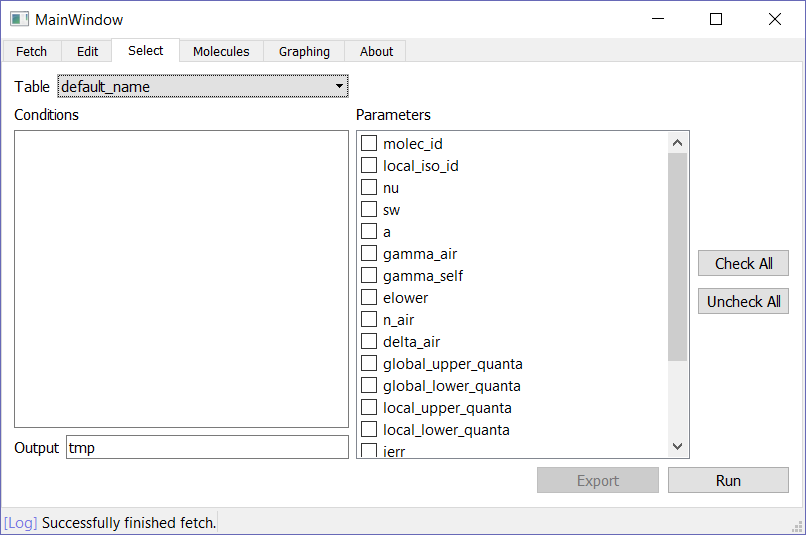
\includegraphics[scale = 0.8]{MainWindow_Select}
Describe select tab

\subsection{Molecules Tab}
The molecules tab provides reference for the available molecules and also reference ids for each molecule.
\begin{center}
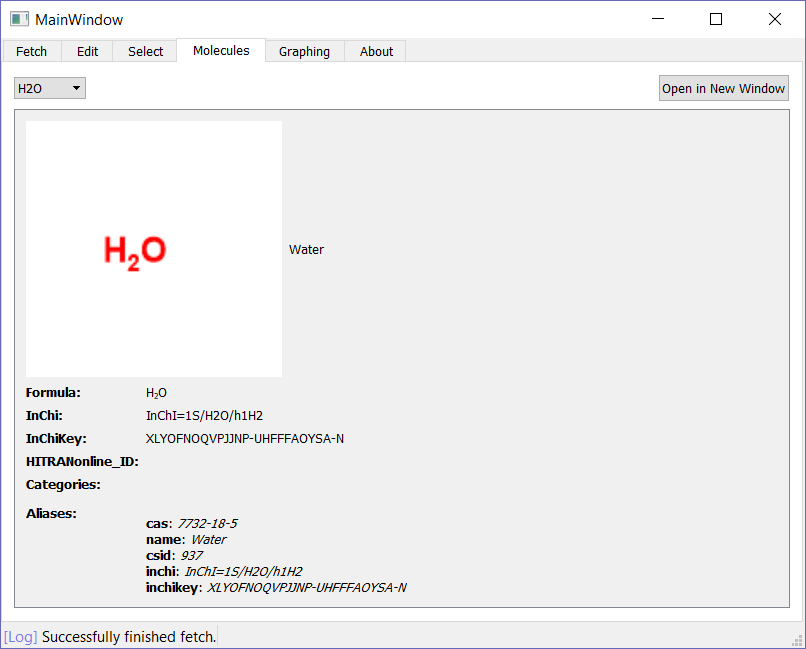
\includegraphics[scale = 0.8]{MainWindow_Molecules}
\end{center}

\subsection{Graphing Tab}
\begin{center}
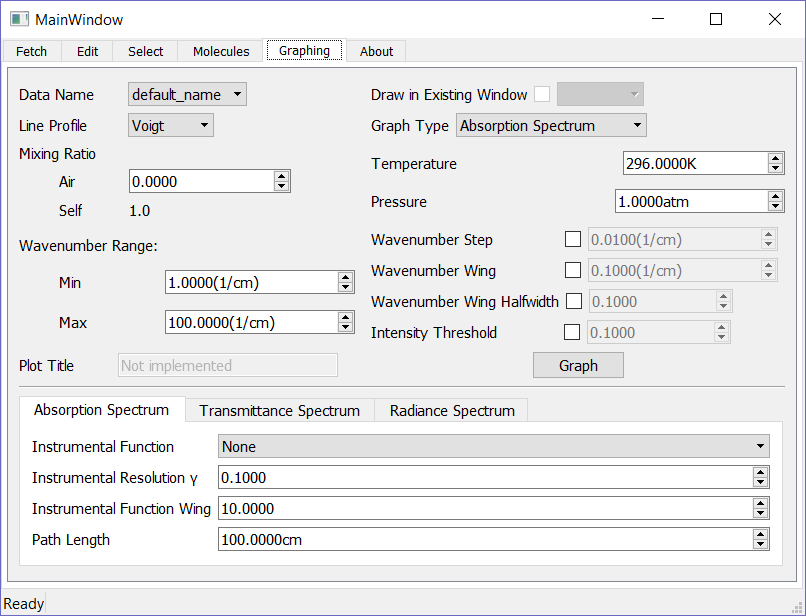
\includegraphics[scale = 0.8]{MainWindow_Graphing}
\end{center}
\subsubsection{Element Dictionary}
\begin{itemize}
\item Data Name - Data file used to plot data.
\item Draw in Existing Window - Checkbox to enable multiple plots on the same graph for the same Line Profiles. List of graph windows open to plot to.
\item Line Profile - List of line profiles, 6 in total.
\item Graph Type - List of types of graphs to produce.
\item Mixing Ratio -
\item Temperature -
\item Pressure -
\item Wave Number Range -
\item Wave Number Step -
\item Wave Number Wing -
\item Wave Number Wing Halfwidth -
\item Intensity Threshold -
\item Plot Title -
\item Graph - Button that creates a plot according to selected parameters.
\end{itemize}

\section{Graphing Window}
\subsection{User Interactivity}
\subsubsection{Box Zoom}
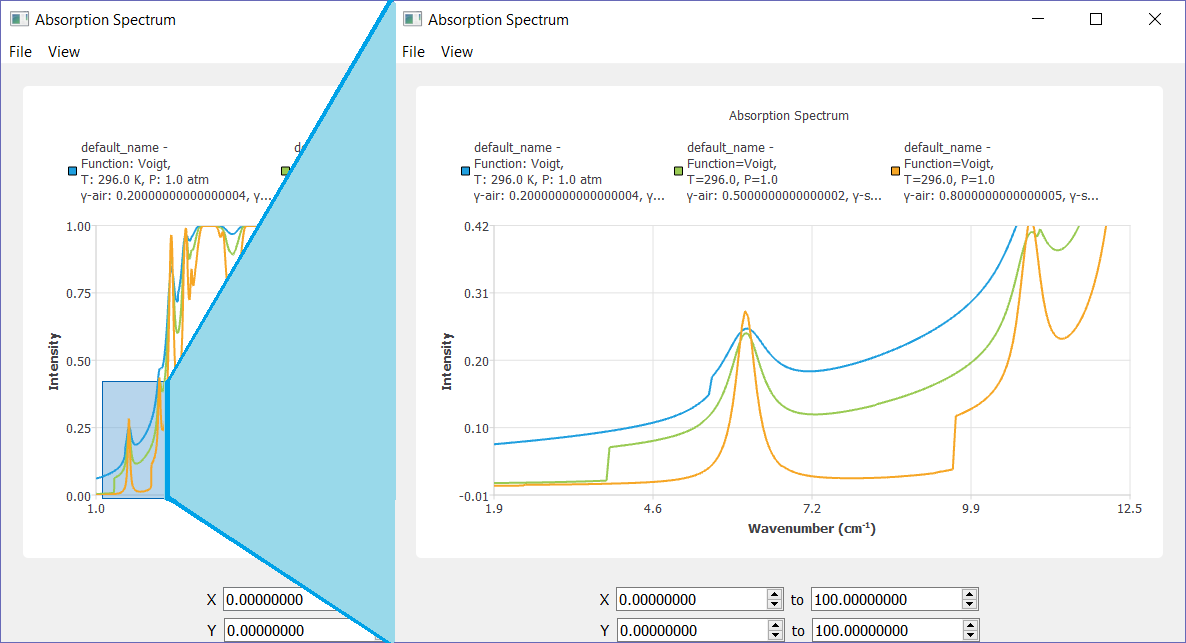
\includegraphics[scale = 0.5]{GraphDemo}
\subsubsection{Save Features}

\section{Demo}
\end{document}
